\documentclass[final]{beamer}

% Use beamerposter with A0 portrait
% \usepackage[size=a0,orientation=landscape,scale=1.05]{beamerposter}
\usepackage[size=a0,orientation=portrait,scale=1.05]{beamerposter}

% Basic packages
\usepackage[utf8]{inputenc}
\usepackage[T1]{fontenc}
\usepackage{lmodern}
\usepackage{graphicx}
\usepackage{booktabs}
\usepackage{multicol}
\usepackage{wrapfig}
\usepackage{natbib}
\bibliographystyle{unsrtnat}

% \usepackage{enumitem} % REMOVED to avoid beamer conflict
\usepackage{hyperref}
\usepackage{array}
\usepackage{ragged2e}
\usepackage{colortbl}
\usepackage{xcolor}
\usepackage{etoolbox} % for safe list tweaks

% Safer list spacing
\makeatletter
\patchcmd{\itemize}{\def\makelabel}{\setlength{\itemsep}{0.4em}\def\makelabel}{}{}%
\patchcmd{\enumerate}{\def\makelabel}{\setlength{\itemsep}{0.4em}\def\makelabel}{}{}%
\makeatother

% Colors
\definecolor{royal}{HTML}{2C3E50}
\definecolor{accent}{HTML}{4A90E2}
\definecolor{softbg}{HTML}{F8F7F4}
\definecolor{danger}{HTML}{C0392B}

\setbeamercolor{normal text}{fg=royal,bg=softbg}
\setbeamercolor{block title}{fg=white,bg=accent}
\setbeamercolor{block body}{fg=royal,bg=white}
\setbeamercolor{alerted text}{fg=danger}
\setbeamercolor{structure}{fg=accent}

\usefonttheme{professionalfonts}
\setlength{\parskip}{0.6em}
\setlength{\parindent}{0pt}
\newcommand{\key}[1]{\textbf{\color{accent}#1}}

% Paper size
% \setlength{\paperwidth}{841mm}
% \setlength{\paperheight}{1189mm}

\title{\LARGE \textbf{Refining the Sunspot Number Series to ISN~V3:\\ Challenges and Benefits for the Space Climate Community}}
\author{\large Kalugodu Chandrashekhar$^{1}$, Laure Lef\`evre$^{1}$, Benjamin Mampaey$^{1}$, Senthamizh Pavai Valliappan$^{1}$, Hisashi Hayakawa$^{2}$, Christian Ritter$^{3}$}
\institute{\large $^{1}$ Royal Observatory of Belgium (ROB), $^{2}$ Nagoya University, $^{3}$ Universit\'e Catholique de Louvain, Louvain-la-Neuve, Belgium}

% Logos (replace with your own files)
\newcommand{\leftlogo}{./logos/observatory_400x332.jpg}
\newcommand{\rightlogo}{./logos/BELSPO_1867x1563.jpg}

% Title box
\setbeamertemplate{headline}{%
  \leavevmode%
  \begin{beamercolorbox}[wd=\paperwidth,ht=5.2cm]{block body}
    \begin{minipage}[c]{0.19\paperwidth}
      \centering \vspace{0.6cm}
      \includegraphics[height=3.6cm]{\leftlogo}
    \end{minipage}%
    \begin{minipage}[c]{0.62\paperwidth}
      \centering \vspace{0.4cm}
%      {\color{royal}\bfseries\fontsize{73}{76}\selectfont FAR\textcolor{accent}{Su}N}\\[0.4cm]
      {\color{royal}\bfseries\fontsize{36}{40}\selectfont \inserttitle}\\[0.3cm]
      {\large \insertauthor}\\[-0.2cm]
      {\normalsize \insertinstitute}
    \end{minipage}%
    \begin{minipage}[c]{0.19\paperwidth}
      \centering \vspace{0.6cm}
      \includegraphics[height=3.6cm]{\rightlogo}
    \end{minipage}
  \end{beamercolorbox}%
}

% Footer
\setbeamertemplate{footline}{%
  \begin{beamercolorbox}[wd=\paperwidth,ht=1.2cm]{block body}
    \hfill \small \textbf{Contact:} your.email@institution \quad|\quad \textbf{Project:} \url{https://www.sidc.be/silso/} \hfill
  \end{beamercolorbox}%
}

% Helper block env
\newenvironment{tightblock}[1]{%
  \begin{block}{#1}\vspace{-0.5em}
}{\end{block}}

\begin{document}
\begin{frame}[t]
\begin{columns}[t,totalwidth=\paperwidth]

% -------- COLUMN 1 --------
\begin{column}{0.32\paperwidth}
\begin{tightblock}{Abstract}
\justifying
The International Sunspot Number (ISN) remains affected by historical scale jumps such as the \emph{Waldmeier break}, even after two major recalibrations. FARSuN (Findability and Accessibility of historical Raw Sunspot Numbers) tackles this by rebuilding the record from the ground up: collecting handwritten logs and tables from 1607--1980, digitizing them, and applying consistent metadata and validation. Early 2025 milestones include integrating the full 1610--1918 \emph{Mittheilungen} corpus, digitizing more than 95\% of the 2\,000+ Zürich observation tables, extracting 338 drawings (1\,056 entries) from the C.\,H. Adams notebooks, and launching quality-control pipelines for the Gruithuisen manuscripts. The reconstructed ISN~V3 will deliver traceable uncertainties, hemispheric indices, and open FAIR-compliant access, strengthening space climate studies, solar cycle prediction, and coupled Sun--Earth research.
\end{tightblock}

\begin{tightblock}{Why Reconstruction?}
  The ISN inherits observer-dependent scale changes (for example the 1947 "Waldmeier jump") that cannot be removed by tweaking coefficients alone. FARSuN pioneers a full reconstruction that replays the entire observing chain.
\begin{itemize}
  \item \textbf{Recalibration} only rescales an existing index; legacy gaps, missing metadata, and hidden assumptions stay baked in.
  \item \textbf{Reconstruction} retrieves the primary artefacts (drawings, tabular logs, weather notes) and recomputes the index with transparent uncertainty tracking.
  \item Direct access to the raw sources lets us audit outliers, model observer response curves, and issue reproducible releases such as ISN~V3.
\end{itemize}
\end{tightblock}

\begin{tightblock}{Four-Axis Methodology}
\begin{enumerate}
  \item \key{Gather Sources}: track down dispersed observing logs (Wolf's \emph{Mittheilungen}, Zürich tables, Gruithuisen manuscripts, Adams drawings) and capture provenance metadata at ingest.
  \item \key{Process Data}: combine handwriting/OCR engines (Transkribus models, custom scripts) with manual double-keying for fragile entries.
  \item \key{Validate \& Standardize}: reconcile aliases, observer IDs, and calendars; model group/spot counting behaviour to derive calibration curves.
  \item \key{Disseminate}: publish machine-readable products, APIs, and VO-ready services with versioned uncertainty bundles for each release.
\end{enumerate}
\end{tightblock}

\begin{tightblock}{FAIR Principles}
  Every dataset and release roadmap is benchmarked against FAIR targets that we monitor with the dashboard shown below.

\begin{itemize}
  \item \textbf{Findable} – persistent DOIs, rich observation-level metadata, and navigable catalogues.
  \item \textbf{Accessible} – open formats (CSV, NetCDF, VO tables) served via HTTPS and scripted download recipes.
  \item \textbf{Interoperable} – shared vocabularies, observer IDs, and VOEvent-ready semantics.
  \item \textbf{Reusable} – versioned releases with uncertainty models, provenance trails, and detailed caveats.
\end{itemize}
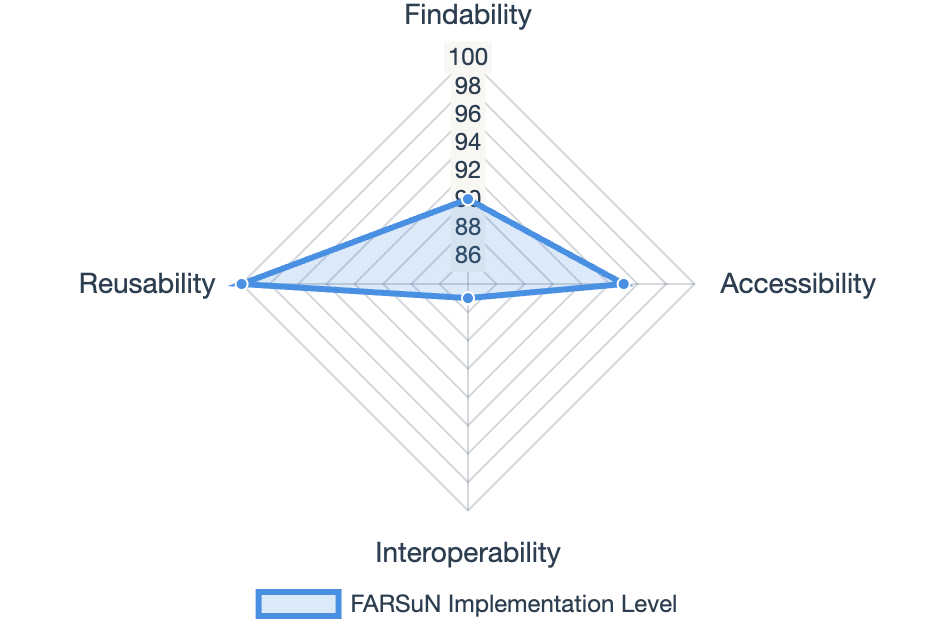
\includegraphics[width=\linewidth]{./figures/fair_radar.png}
\end{tightblock}
\end{column}

% -------- COLUMN 2 --------
\begin{column}{0.32\paperwidth}
\begin{tightblock}{Key Datasets}
\begin{tabular}{@{}p{0.33\linewidth}p{0.23\linewidth}p{0.38\linewidth}@{}}
\toprule
\textbf{Source} & \textbf{Period} & \textbf{Current Focus} \\ \midrule
Zürich Tables & 1945--1979 & 95\% of 2\,000+ tables digitized; metadata encoding for late-1970s observers underway. \\
\emph{Mittheilungen} & 1610--1918 & Fully integrated; observer statistics produced from 400+ years of entries. \\
Gruithuisen Manuscripts & 1817--1849 & 25\% transcription via Transkribus; file renaming algorithm + dual QC for group/spot counts. \\
C. H. Adams Drawings & 1819--1823 & 338 sketches extracted (1\,056 entries); spotless days cross-checked against Wolf series. \\
Augustin Stark Ledgers & 1813--1835 & Normalizing tabular layouts; linking weather annotations to group counts. \\
Rost Journals & 18th--19th c. & Building metadata vocabularies prior to digitization ingest. \\
\bottomrule
\end{tabular}
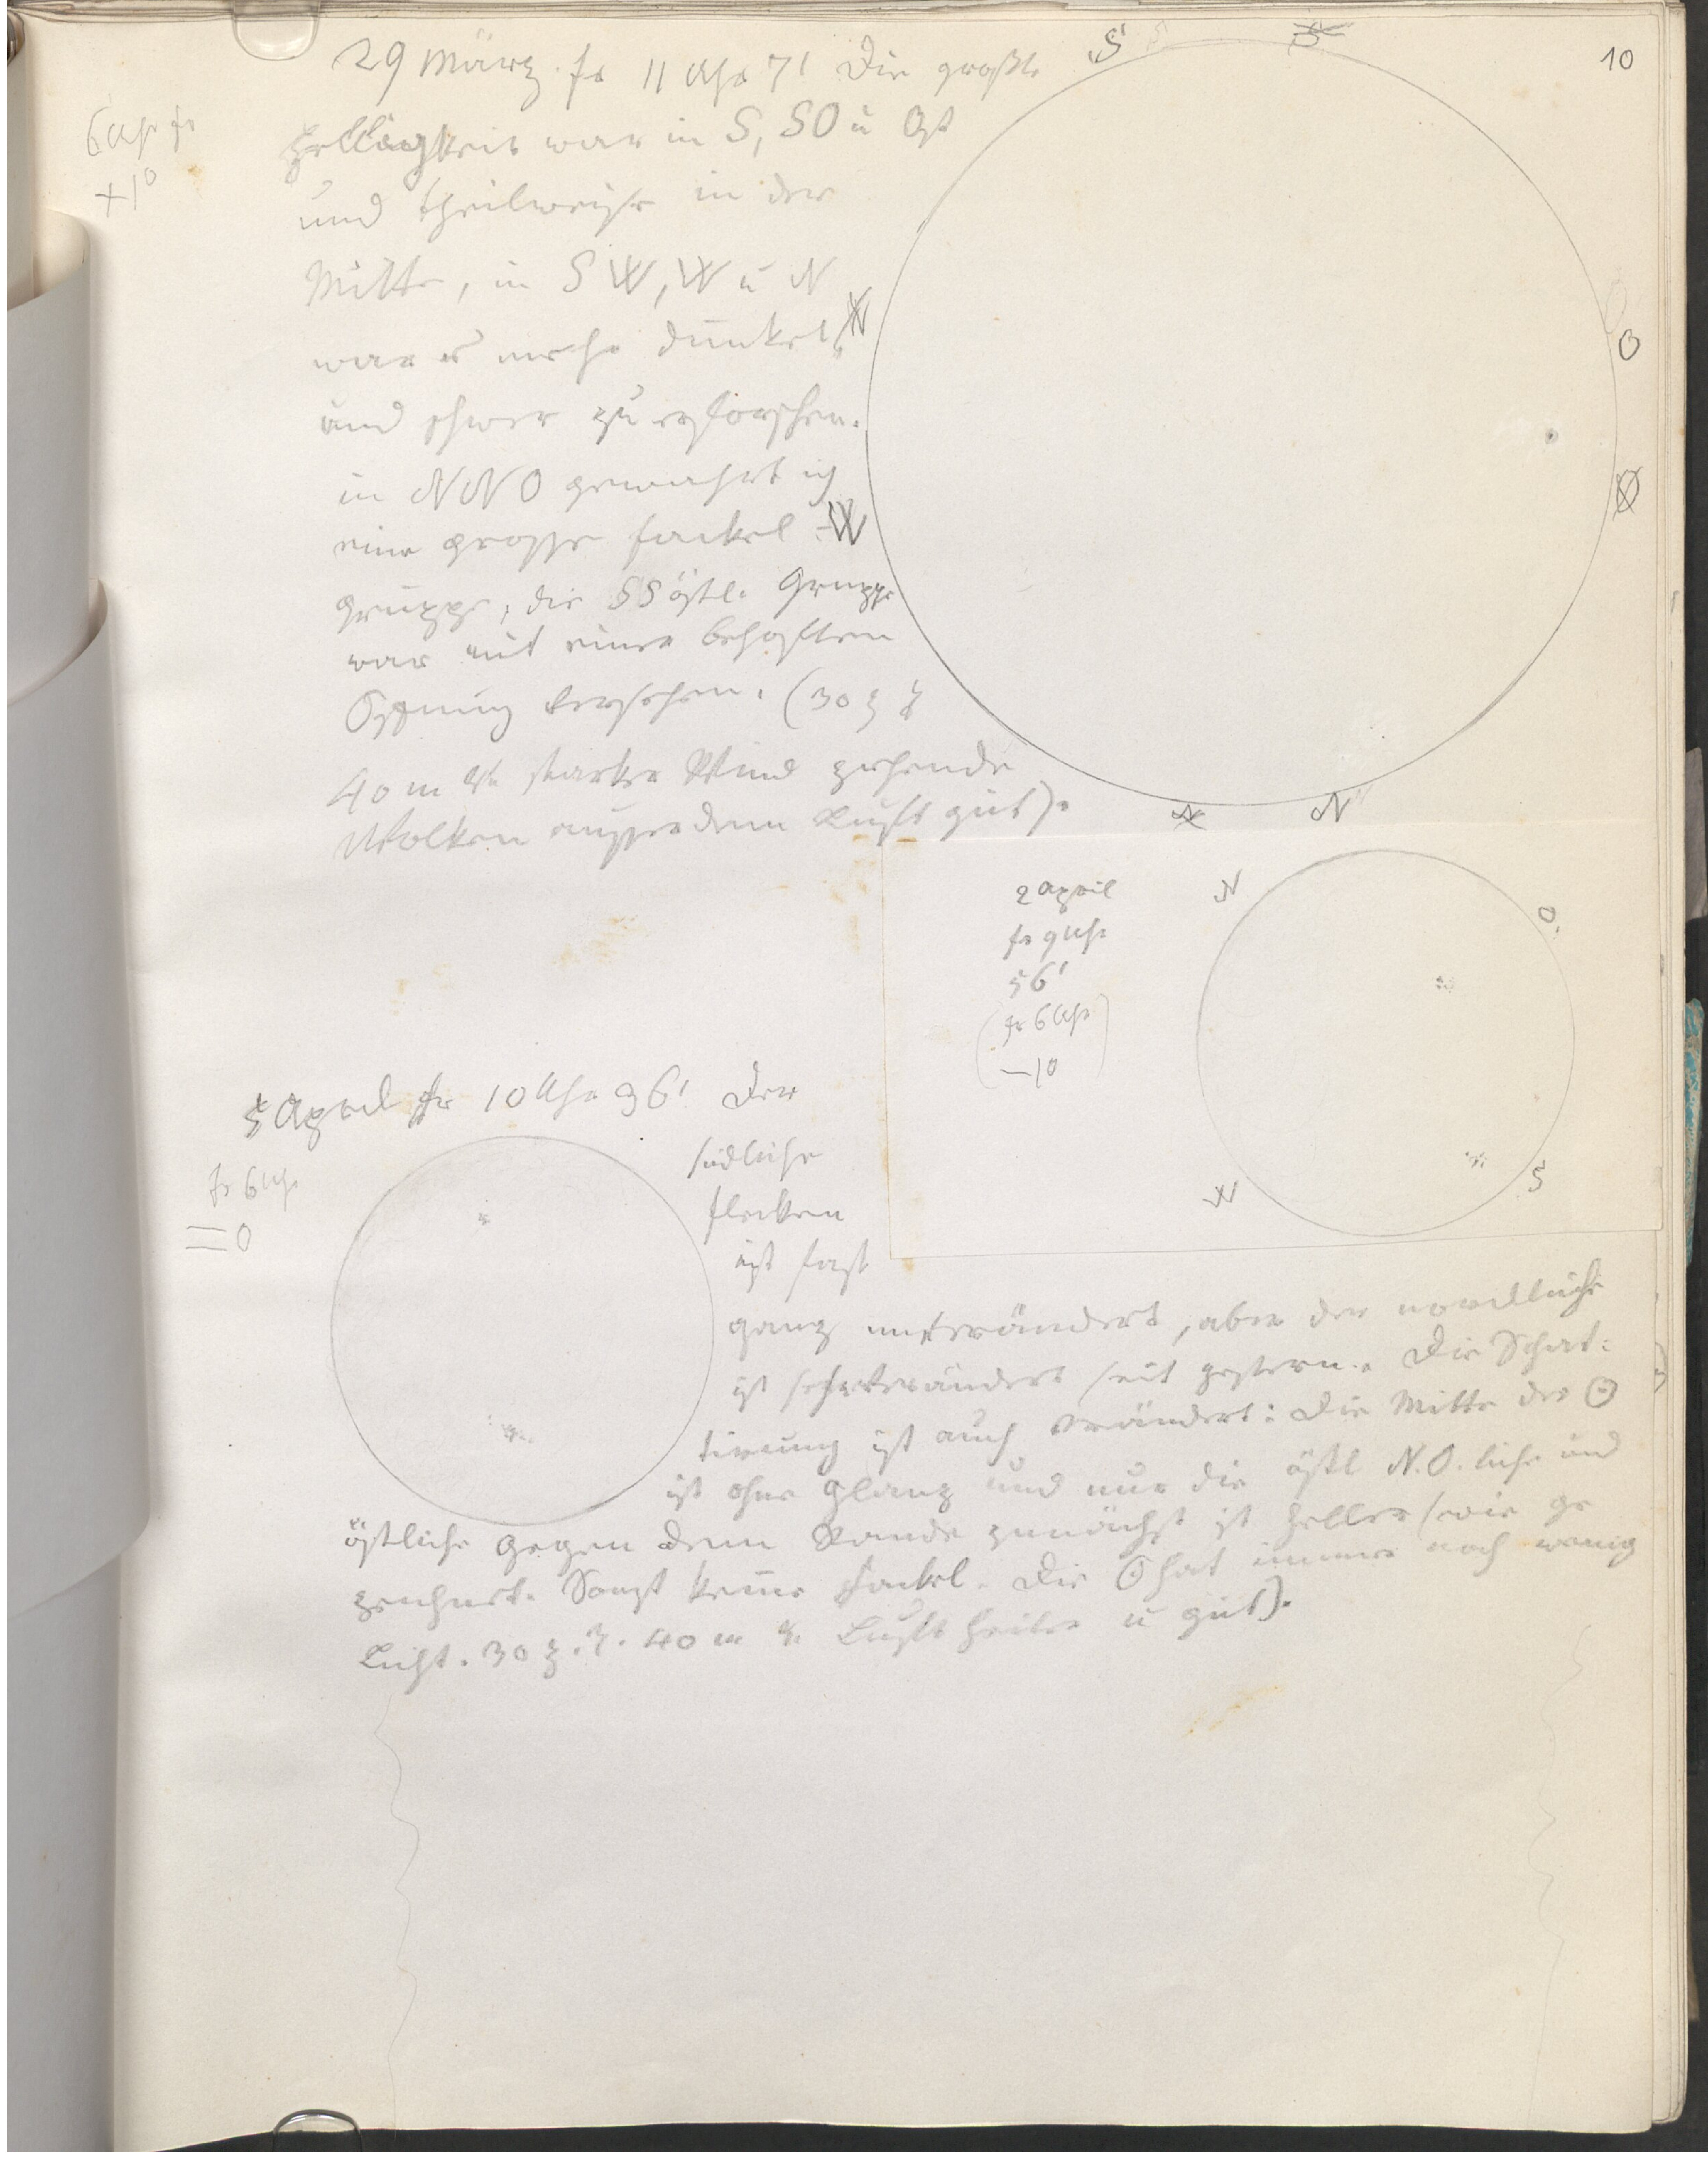
\includegraphics[width=0.5\linewidth]{./figures/gruithuisen/sample1.jpg}
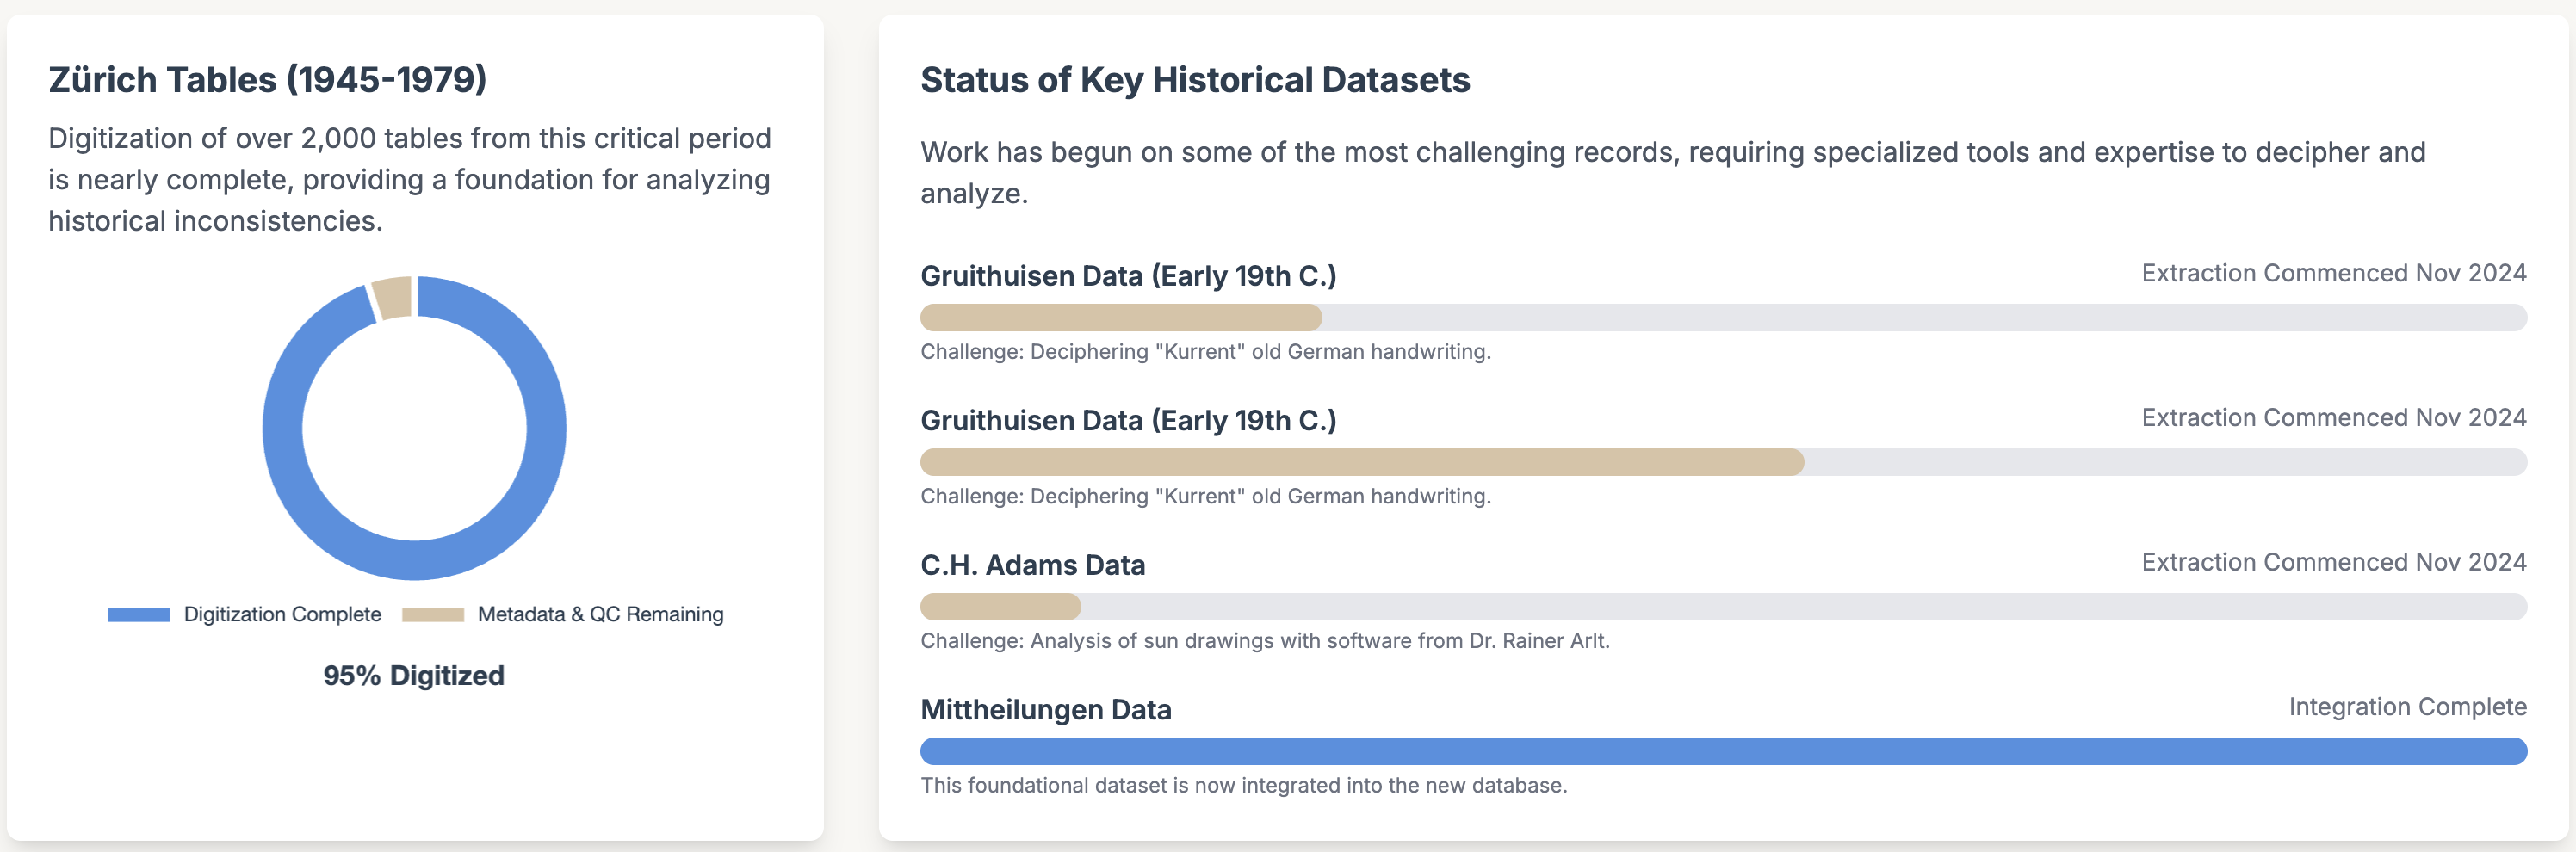
\includegraphics[width=\linewidth]{./figures/dataset_progress.png}
\end{tightblock}

\begin{tightblock}{Progress Highlights (Early 2025)}
\begin{itemize}
  \item Citizen-science ready interface blueprint finished; aligns with planned public transcription portal.
  \item Zürich production line blends Transkribus-assisted extraction with manual review to hit 2025 completion.
  \item Gruithuisen workflow pairs Kurrent script specialists with validation scripts to flag missing sun symbols.
  \item Adams drawings compared against \emph{Mittheilungen} daily records to benchmark spotless-day agreement.
\end{itemize}
\end{tightblock}

\begin{tightblock}{Observer Timeline}
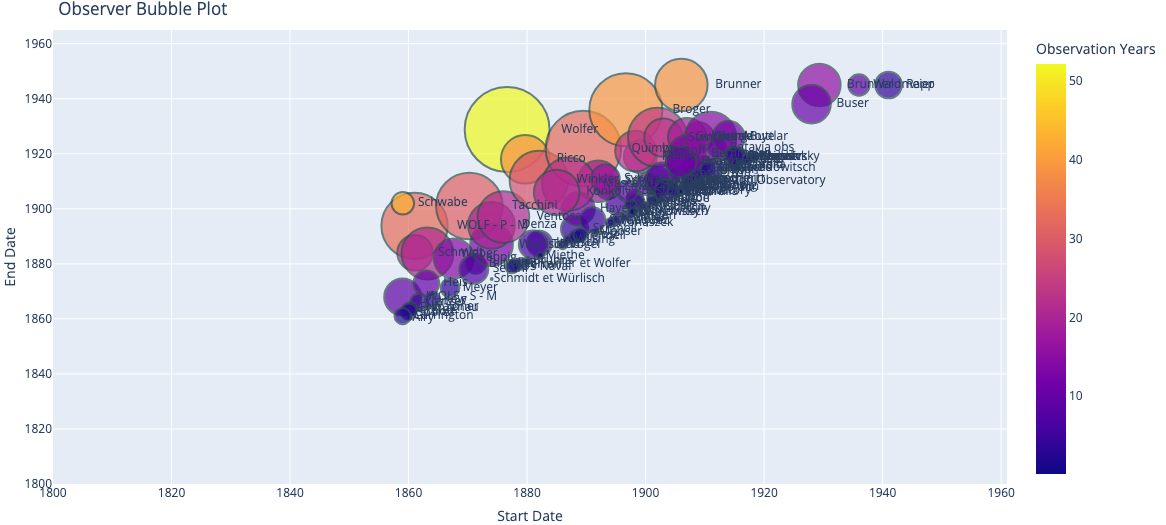
\includegraphics[width=\linewidth]{./figures/observers_bubble.png}
\scriptsize (Bubble size = total observations; color = years)
\end{tightblock}

\begin{tightblock}{Methods}
\begin{itemize}
  \item Dual-mode transcription: tailored Transkribus handwriting models plus manual keying for complex tables.
  \item Data hygiene: observer alias reconciliation, calendar conversions, and spot/group recount audits.
  \item Uncertainty modelling: propagate observer calibration curves and note spotless-day confidence flags.
  \item Automation: reproducible Python pipelines with checkpoints for citizen-science ingestion and review.
\end{itemize}
\end{tightblock}
\end{column}

% -------- COLUMN 3 --------
\begin{column}{0.32\paperwidth}
\begin{tightblock}{From Raw to ISN V3}
\begin{enumerate}
  \item Curate daily counts with provenance-rich metadata (observer, instrument, weather context).
  \item Solve observer response functions to align group/spot scales across centuries.
  \item Aggregate to monthly, yearly, and hemispheric indices with propagated uncertainties.
  \item Benchmark against ISN~V2 and satellite-era proxies to validate drift corrections.
\end{enumerate}
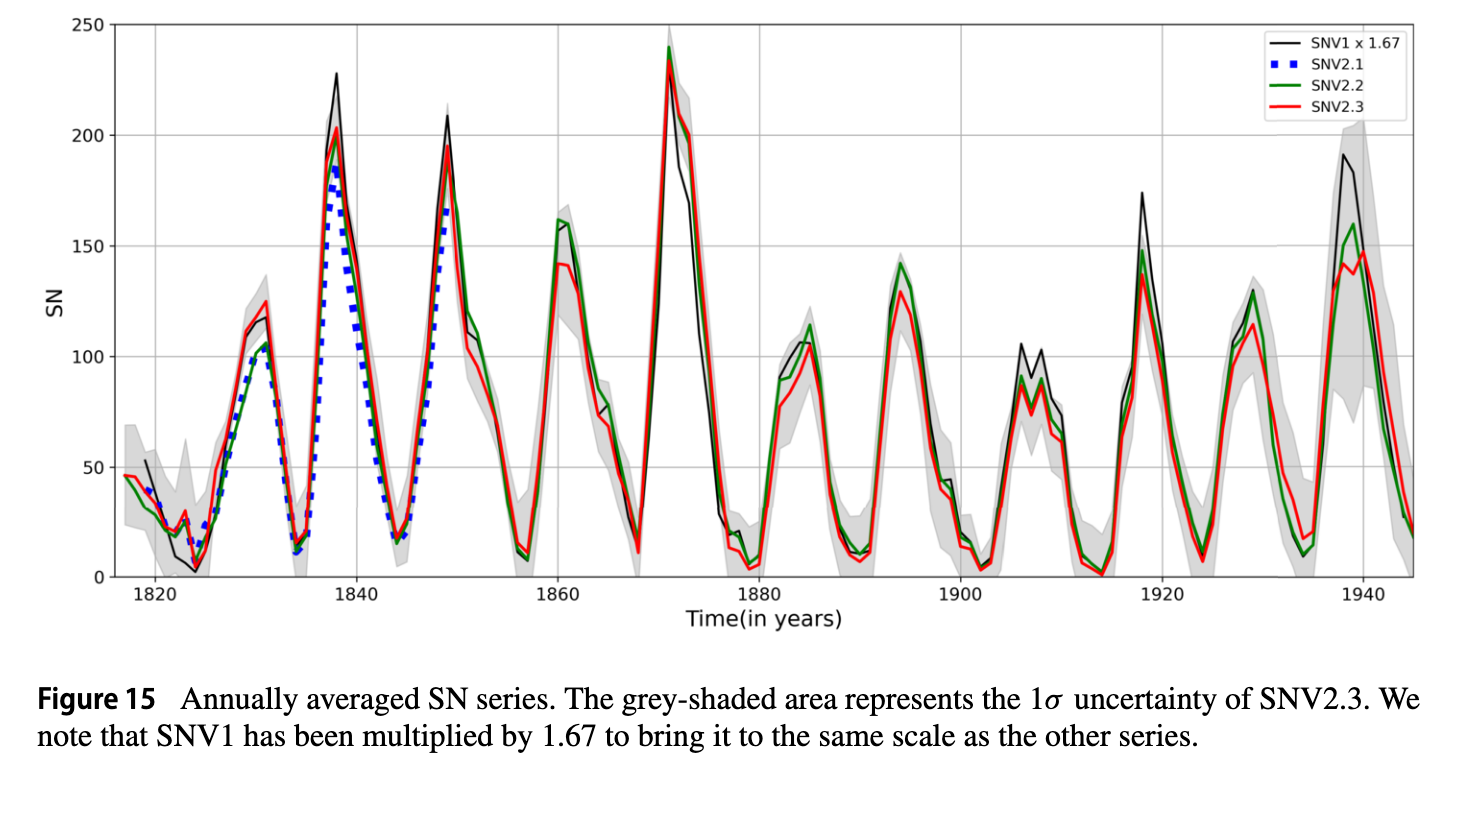
\includegraphics[width=0.9\linewidth]{./figures/comparison_panel.png}
\end{tightblock}

\begin{tightblock}{Challenges}
\begin{itemize}
  \item Deciphering \emph{Kurrent} manuscripts and annotating non-solar notes without losing context.
  \item Harmonising heterogeneous formats (drawings, tabular ledgers, weather marginalia).
  \item Quantifying observer bias and spotless-day reporting habits over centuries.
  \item Maintaining end-to-end provenance from scanned folio to released data product.
\end{itemize}
\end{tightblock}

\begin{tightblock}{Impact}
\begin{itemize}
  \item Citizen science engagement accelerates transcription and STEM outreach.
  \item Improved solar cycle prediction skill via unbiased long-term baselines.
  \item Reference climatology for operational space weather services.
  \item Higher-fidelity forcing inputs for Earth system and climate models.
\end{itemize}
\end{tightblock}

\begin{tightblock}{Outlook}
\begin{itemize}
  \item Launch citizen-science transcription portal with tailored training sets.
  \item Publish ISN~V3 release notes with uncertainty budget and API endpoints.
  \item Expand collaborations (Nagoya, UCLouvain, ROB) for cross-validation and joint publications.
\end{itemize}
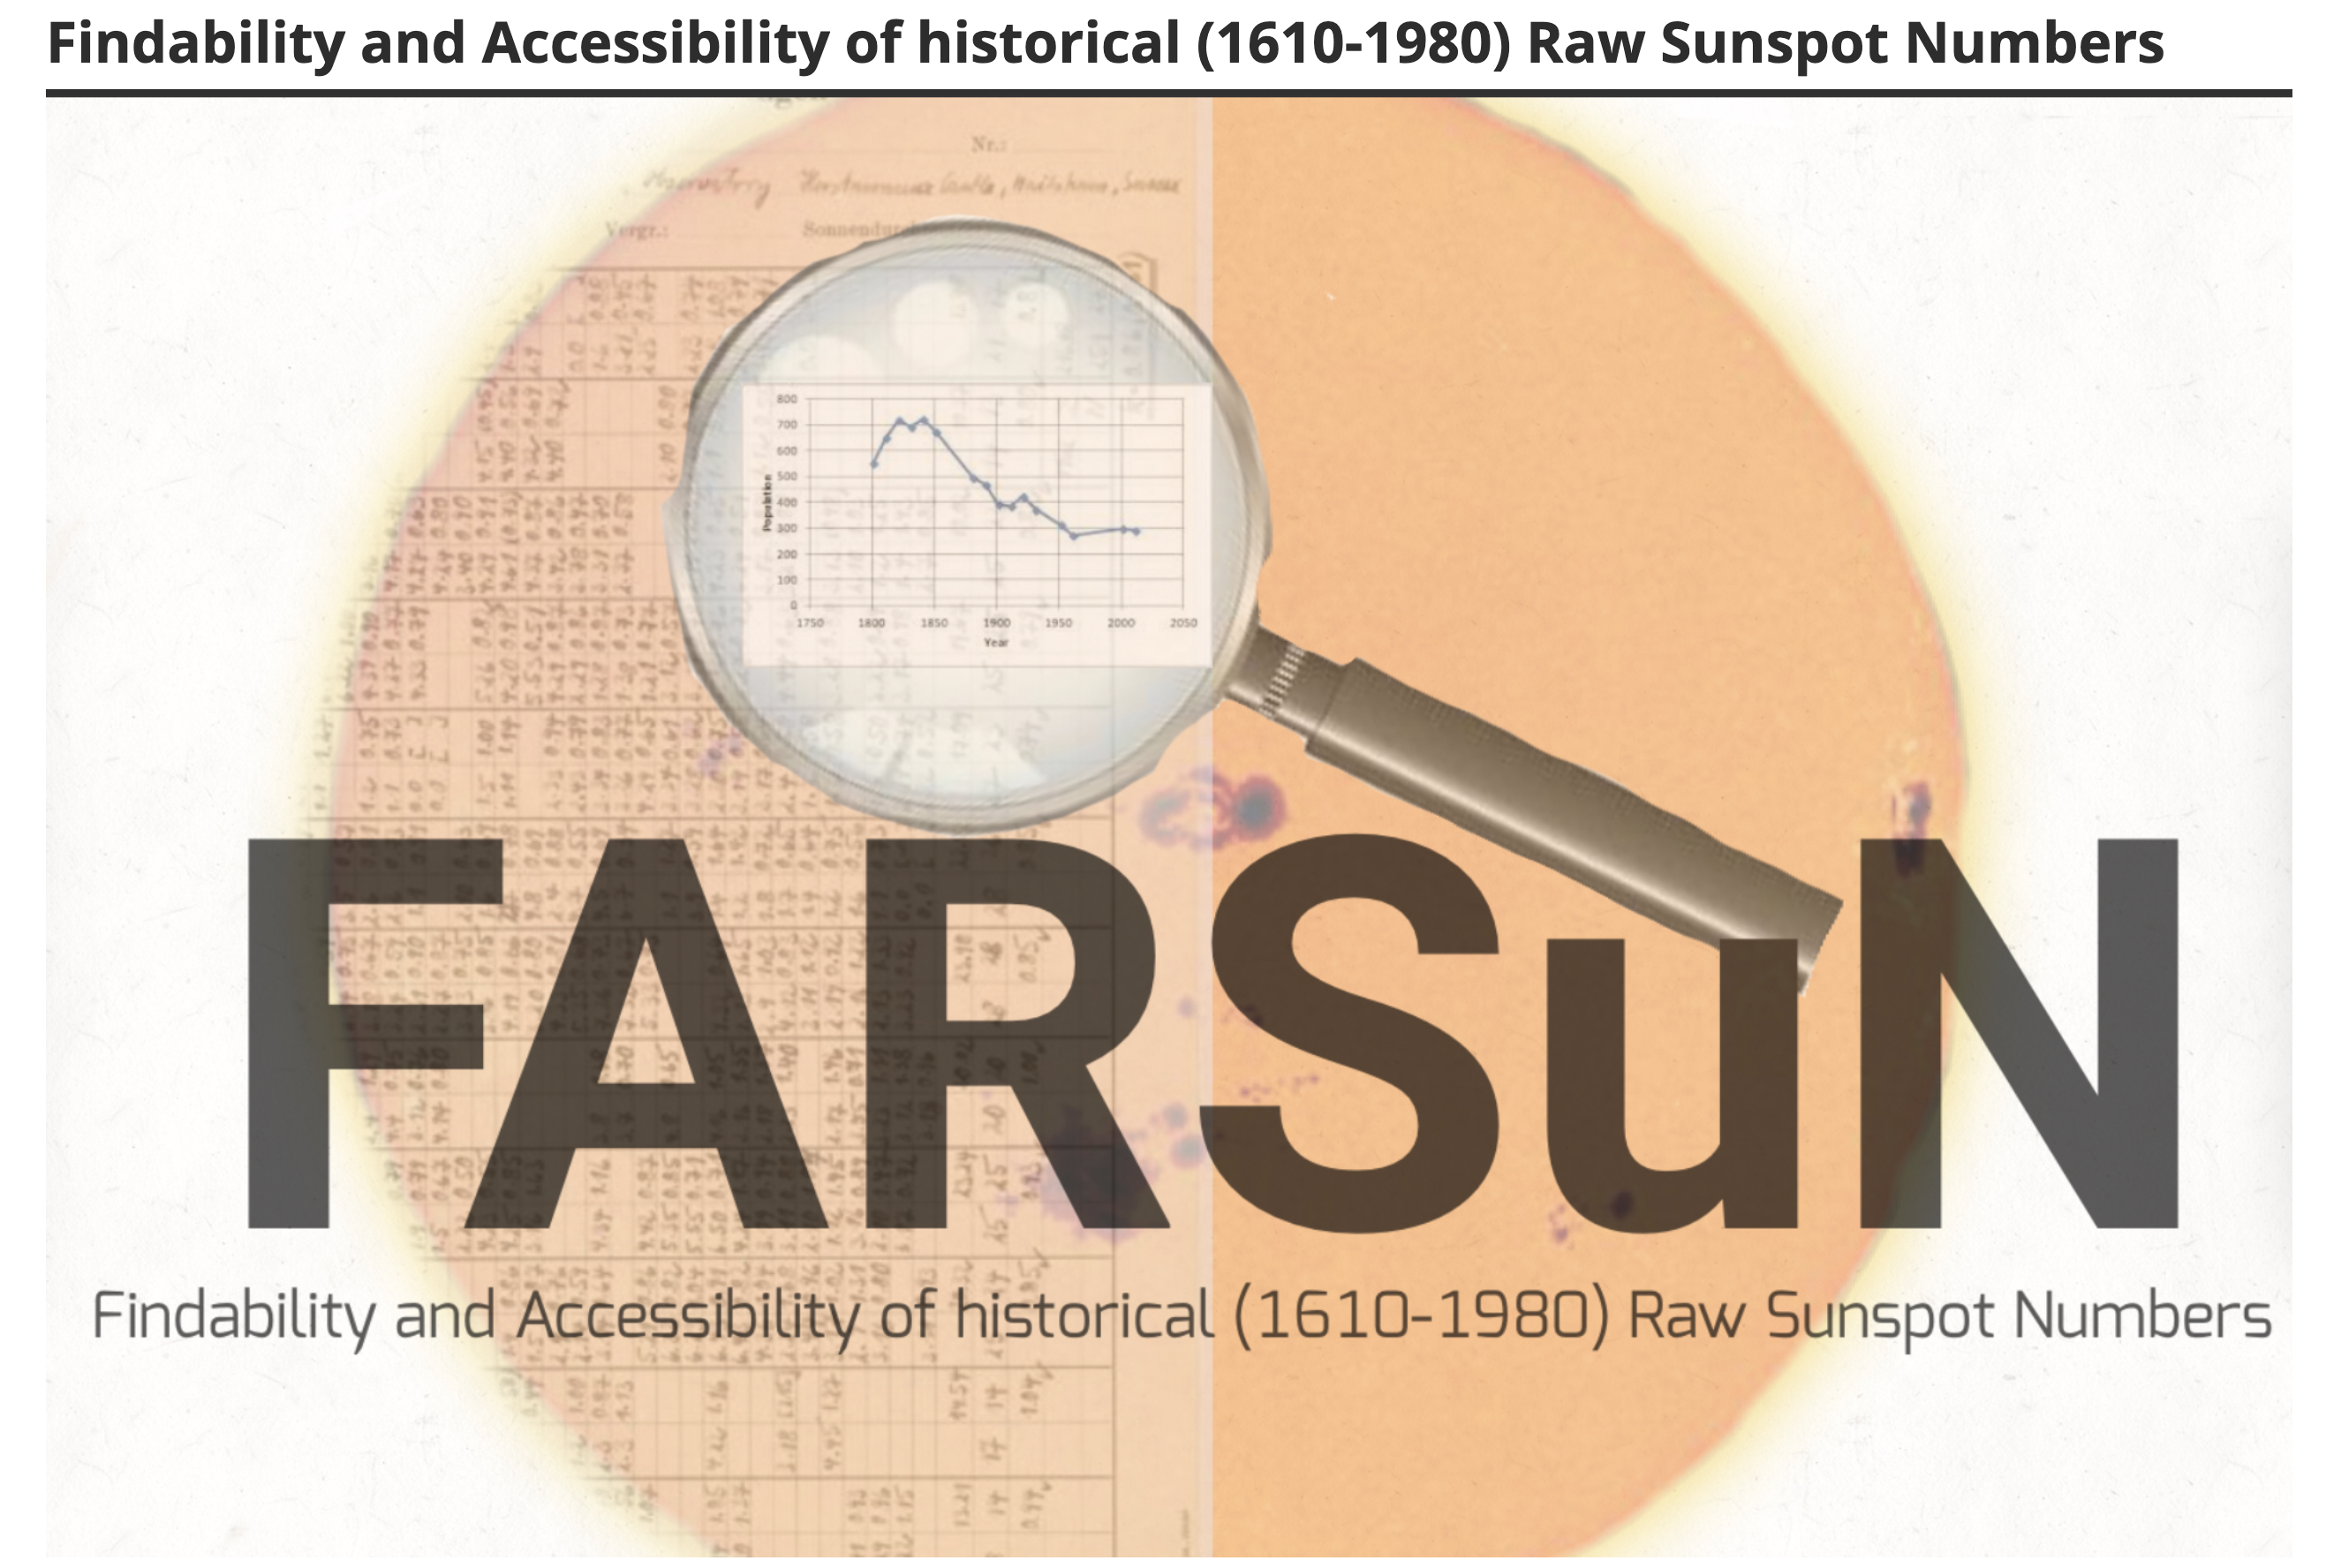
\includegraphics[width=0.8\linewidth]{./figures/ack_.png}
\end{tightblock}

\begin{tightblock}{References}
{\footnotesize \bibliography{articles}}
\end{tightblock}
\end{column}

\end{columns}
\end{frame}
\end{document}
